\documentclass[graybox]{svmult}
%\usepackage{mathptmx}       % selects Times Roman as basic font
%\usepackage{helvet}         % selects Helvetica as sans-serif font
%\usepackage{courier}        % selects Courier as typewriter font
%\usepackage{type1cm}        % activate if the above 3 fonts are
                            % not available on your system
%
%\usepackage{makeidx}         % allows index generation
\usepackage{graphicx}        % standard LaTeX graphics tool
                             % when including figure files
%\usepackage{multicol}        % used for the two-column index
%\usepackage[bottom]{footmisc}% places footnotes at page bottom
\usepackage{amsfonts, amssymb}

%\makeindex             % used for the subject index
                       % please use the style svind.ist with
                       % your makeindex program

%%%%%%%%%%%%%%%%%%%%%%%%%%%%%%%%%%%%%%%%%%%%%%%%%%%%%%%%%%%%%%%%%%%%%%%%%%%%%%%%%%%%%%%%%

\newcommand{\dom}{\mathop{\rm dom}}
\renewcommand{\Im}{\mathop{\rm Im}}
\newcommand{\supp}{\mathop{\rm supp}}
\newcommand{\sgn}{\mathop{\rm sgn}}
\newcommand{\rank}{\mathop{\rm rank}}
\renewcommand{\kappa}{\varkappa}
\newcommand{\rmi}{{\rm i}}
\newcommand{\Real}{\mathbb R}
\newcommand{\eps}{\varepsilon}
\newcommand{\en}{{\nu,\eps}}
\newcommand{\cI}{\mathcal{I}}
\newcommand{\mv}[1]{\langle #1 \rangle_0}
\newcommand{\fm}[1]{\langle #1 \rangle_1}
\newcommand{\fpr}[1]{{#1}^{(-1)}}
\newcommand{\spr}[1]{{#1}^{(-2)}}
\newcommand{\ra}{\rangle}
\newcommand{\la}{\langle}
\newcommand{\fra}{\mathfrak{a}}

% MATH -----------------------------------------------------------
\newcommand{\norm}[1]{\left\Vert#1\right\Vert}
\newcommand{\abs}[1]{\left\vert#1\right\vert}
\newcommand{\set}[1]{\left\{#1\right\}}
\newcommand{\To}{\longrightarrow}
\newcommand{\BX}{\mathbf{B}(X)}
\newcommand{\A}{\mathcal{A}}
% ----------------------------------------------------------------


\newcommand{\mg}[1]{{\color{magenta}{#1}}}
\newcommand{\rd}[1]{{\color{red}{#1}}}
\renewcommand{\emph}[1]{{\textit{#1}}}
\renewcommand{\phi}{\varphi}
\newcommand\rmd{\mathrm{d}}
\newcommand\rme{\mathrm{e}}
\newcommand\rmR{\mathrm{R}}
\renewcommand{\leq}{\leqslant}
\renewcommand{\geq}{\geqslant}
\newcommand{\myIm}{\mathop{\rm Im}}
\newcommand{\myRe}{\mathop{\rm Re}}
\newcommand{\sign}{\mathop{\rm sign}}
\newcommand{\ess}{\mathop{\rm ess}}
\newcommand{\bl}[1]{{\color{blue}{#1}}}
\newcommand{\oB}[1]{\langle{#1},g\rangle\hskip1pt f+\langle{#1},f\rangle\hskip1pt g}
\newcommand\nep{\textstyle\frac n\eps}
\newcommand\te{\left(\frac t\eps\right)}
\newcommand\se{\left(\frac s\eps\right)}
\newcommand\pfg{p}
\newcommand\hy{\hat{y}_\eps}
\newcommand{\eqref}[1]{(\ref{#1})}
\newcommand{\pte}{\partial_\tau}
\newcommand{\pts}{\partial_s}

\begin{document}

\title*{Schr\"{o}dinger operators with}
%\titlerunning{Short Title}
\author{Yuriy Golovaty}
%\authorrunning{Short Title}
\institute{Yuriy Golovaty \at Ivan Franko National University of Lviv,
1, Universytetska str., Lviv, 79000, Ukraine \\ \email{yuriy.golovaty@lnu.edu.ua}}

\maketitle

\abstract*{Each chapter should be preceded by an abstract (10--15 lines long) that summarizes the content. The abstract will appear \textit{online} at \url{www.SpringerLink.com} and be available with unrestricted access.}

\abstract{Each chapter should be preceded by an abstract (10--15 lines long) that summarizes the content. The abstract will appear \textit{online} at \url{www.SpringerLink.com} and be available with unrestricted access. }

\section{Introduction: What is the Difference between $\delta$ and $\delta'$ Potentials?    }
\label{Sec:Introduction}


\section{Statement of Problem and Main Results}
\label{Sec:Statment}

Let us consider the family of operators
\begin{equation}\label{OprHe}
H_\eps=-\Delta +W(x)+V_\eps(x).
\end{equation}
Suppose that the unperturbed operator $H_0=-\Delta +W(x)$ is self-adjoint in $L^2(\Real^2)$ with a domain $\dom H_0$. In addition, we assume that the potential $W$ belongs to $L^\infty_{loc}(\Real^2)$.

Let $\gamma$ be a  closed $C^2$-curve without self-intersection
points. We will denote by $\omega_\eps$ the $\eps$-neighborhood of $\gamma$, i.e., the union of all open balls with radius $\eps$ and center on~$\gamma$. Consider $\eps$ sufficiently small such that boundary
$\partial\omega_\eps$ is smooth. Without loss of generality we can assume that it holds for $\eps\in (0,1)$. We also suppose that potentials $V_\eps$ have compact supports that lie in $\omega_\eps$. Therefore the supports of $V_\eps$ shrink to curve $\gamma$ as $\eps\to 0$.

\paragraph{Local coordinates}
To specify  the dependence of $V_\eps$ on the small parameter  we introduce  local coordinates in $\omega_\eps$. Let $\alpha\colon\; S\to \Real^2$ be the unit-speed $C^2$-parametrization of $\gamma$ with the natural parameter $s\in S$. Here $S$ is a circle of the same length as the length of $\gamma$.  Also
the vector $\nu=(-\dot{\alpha}_2, \dot{\alpha}_1)$ is the unit normal on $\gamma$, because  $\|\dot{\alpha}\|=1$.
We define the local coordinates $(s,n)$ in $\omega_\eps$ by
\begin{equation}\label{LocalTr}
    x=\alpha(s)+n\nu(s), \qquad (s,n)\in S\times (-\eps, \eps).
\end{equation}
Therefore  $\omega_\eps$ is diffeomorphic to cylinder $Q_\eps=S\times(-\eps,\eps)$ for $\eps$ small enough.

The coordinate $n$ can be regarded as the signed distance from a point $x$ to $\gamma$. The Jacobian of transformation (\ref{LocalTr}) is given by
\begin{eqnarray}\nonumber
J(s,n)&&=
\left|
        \begin{array}{cr}
          \dot{\alpha}_1(s)-n\ddot{\alpha}_2(s)\phantom{0} &  -\dot{\alpha}_2(s)\\
          \dot{\alpha}_2(s)+n\ddot{\alpha}_1(s)\phantom{0} & \dot{\alpha}_1(s)\\
        \end{array}
      \right|\\\nonumber
&&=\dot{\alpha}_1^2(s)+\dot{\alpha}_2^2(s)
-n\big(\dot{\alpha}_1(s)\ddot{\alpha}_2(s)-
  \dot{\alpha}_2(s)\ddot{\alpha}_1(s)\big)=1-n \kappa(s),
\end{eqnarray}
where $\kappa=\det(\dot{\alpha},\ddot{\alpha})$ is the signed curvature of $\gamma$. Hence, $J$ is positive for sufficiently small $\eps$, because $|n|<\eps$ and the curvature $\kappa$  is  bounded on $\gamma$.



Metric tensor $g=(g_{ij})$ of $\omega_\eps$ in the orthogonal coordinates has the form
$$
    g=\left(
        \begin{array}{cc}
          J^2\phantom{0} & 0 \\
          0\phantom{0} & 1\\
        \end{array}
      \right),
$$
In fact, we have $g_{11}=x_n\cdot x_n=|\nu|^2=1$ and $g_{22}=x_s\cdot x_s=|\dot{\alpha}+n \dot{\nu}|^2
=|(1-n\kappa) \dot{\alpha}|^2=J^2$, by the Frenet-Serret formula $\dot{\nu}=-\kappa \dot{\alpha}$.
In the local coordinates $(s,n)$ the gradient and the Laplacian become
\begin{eqnarray}\nonumber
&\nabla \phi=J^{-1}\partial_s\phi\, \dot{\alpha}+\partial_n\phi\, \nu\\
\label{LaplacianInSN}
&\Delta \phi=J(s,n)^{-1}\left(\partial_s(J(s,n)^{-1}\partial_s \phi)+ \partial_n(J(s,n)\partial_n \phi)\right)
\end{eqnarray}
as is easy to check.  Therefore we have
\begin{equation}\label{ScalarProdGrads}
  \nabla \phi\cdot \nabla \psi=J^{-2}\partial_s\phi \partial_s \psi+
\partial_n \phi \partial_n \psi.
\end{equation}

\begin{figure}[h]
\centering
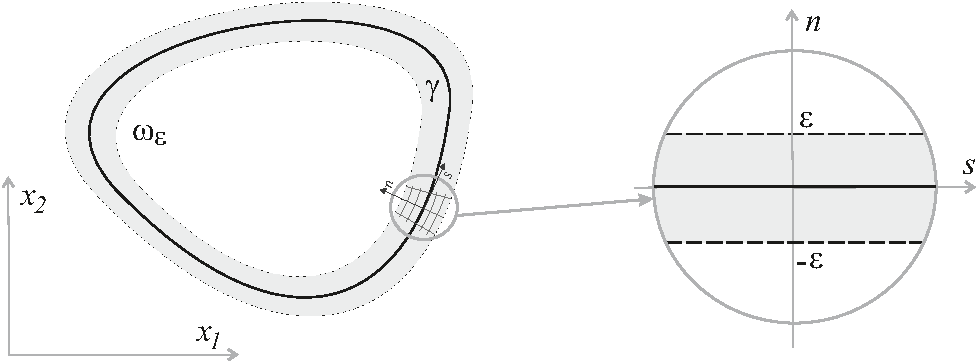
\includegraphics[scale=.6]{LocalCoords}
\caption{Local coordinates in the $\eps$-neighbourhood of $\gamma$.}
\label{FigLocalCoords}
\end{figure}


We suppose that the localized potential has the following structure
\begin{equation}\label{Veps}
V_\eps(x)=\frac{1}{\eps^2}\,V\left(\frac{n}{\eps}\right),
\end{equation}
where $V$ is a $L^\infty(\Real)$-function such that $\supp V\subset [-1,1]$. The key assumption is that $V$ does not depend on the local coordinate $s$.

If $V$ has the zero mean, then
$$
   V_\eps(x)\to \beta\left(\partial_\nu\delta_\gamma+\kappa \delta_\gamma\right)
$$
in the sense of distributions, where $\delta_\gamma$ is Dirac's delta function supported on $\gamma$ and
$$
  \beta=-\int_\Real xV(x)\,dx.
$$
Otherwise sequence $V_\eps$ diverges in the space of distributions.
In fact, for any $\phi\in C^\infty_0(\Real^2)$ we have
\begin{eqnarray}\nonumber
&&\int_{\Real^2}V_\eps(x)\phi(x)\,dx=
\frac{1}{\eps^2}\int_{-\eps}^{\eps}\int_0^\ell V\left(\frac{n}{\eps}\right)\phi(s,n)(1-n\kappa(s))\,ds\,dn\\\nonumber
&&=\frac{1}{\eps^2}\int_{-\eps}^{\eps}\int_0^\ell V\left(\frac{n}{\eps}\right)\left(\phi(s,0)+(\partial_n\phi(s,0)-\kappa(s)\phi(s,0))n+O(n^2)\right)\,ds\,dn
\\\nonumber
&& =\frac{1}{\eps}\int_{-1}^1 V(t)\,dt \int_0^\ell\phi(s,0)\,ds+
\int_{-1}^1 t V(t)\,dt \int_0^\ell(\partial_n\phi(s,0)-\kappa(s)\phi(s,0))\,ds+O(\eps)
\\\nonumber
&&\qquad\qquad\qquad\qquad\to \beta\int_\gamma\left(\partial_\nu\delta_\gamma+\kappa \delta_\gamma\right)\phi\,d\gamma\quad \hbox{as }\eps\to 0,
\end{eqnarray}
since $V$ is a function of zero mean.

\paragraph{ Zero Energy Resonances and Half-Bound States}
We set  $h_\pm=\lim_{x\to\pm\infty}h(x)$ and
\begin{equation}\label{Theta}
  \theta= \frac{h_+}{h_-}.
\end{equation}

\section{Proof of Theorem}
\label{Sec:Proof}
\subsection{Limit Operator}
Given $f\in L_2(\Real^2)$ and $\zeta\in \mathbb{C}$ with  $\Im\zeta\neq0$, we set
\begin{equation}\label{Ueps}
u_\eps=(H_\eps-\zeta)^{-1}f.
\end{equation}
Let us find a formal asymptotics of $u_\eps$, as $\eps\to 0$, in the form
\begin{equation}\label{AsymptoticsUe}
w_\eps(x)=
\left\{
  \begin{array}{ll}
    u(x)&\quad \hbox{in \ }\Real^2\setminus \omega_\eps, \\
    v_0\left(s,\nep\right)+\eps v_1\left(s,\nep\right)+\eps^2 v_2^\eps\left(s,\nep\right)
&\quad \hbox{in \ } \omega_\eps.
  \end{array}
\right.
\end{equation}
We denote by $\gamma_t=\{x\in\Real^2\colon\; x=\alpha(s)+t\nu(s), \; s\in S\}$ the closed curve that is obtained from $\gamma$ by flowing for ``time'' $t$ along the normal vector field. Then the boundary of $\omega_\eps$ consists of two $C^2$-curves $\gamma_{-\eps}$ and $\gamma_{\eps}$.
We will match two different approximations by conditions
\begin{equation}\label{MatchingCnds}
  [u_\eps]_{\gamma_{\pm\eps}}=0, \qquad [\partial_\nu u_\eps]_{\gamma_{\pm\eps}}=0,
\end{equation}
where $[\,\cdot\,]_{\gamma_{\pm\eps}}$ is a jump  across $\gamma_{\pm\eps}$.
Since function $u_\eps$ solves equation
\begin{equation}\label{EqnUe}
-\Delta u_\eps +(W+V_\eps-\zeta) u_\eps= f\quad \hbox{in \ } \Real^2
\end{equation}
and potentials $V_\eps$ shrink to $\gamma$,
the leading term $u$ must be a solution of
$$
-\Delta u+(W-\zeta)u= f \quad \hbox{in \ } \Real^2\setminus \gamma,
$$
subject to appropriate interface conditions on $\gamma$. To find these conditions, we consider equation \eqref{EqnUe} in the local coordinates $(s,\tau)$, where $\tau=n/\eps$.
According to \eqref{LaplacianInSN} the Laplacian
can be written as
%\begin{equation}
%  \Delta =\eps^{-2}J_\eps(s,\tau)^{-1}\Big( \partial_\tau
%\left(J_\eps(s,\tau)\partial_\tau\right) +\eps^2\partial_s
%\left(J_\eps(s,\tau)^{-1}\partial_s\right) \Big),
%\end{equation}
\begin{equation}
  \Delta =\frac1{1-\eps \tau\kappa}\left( \eps^{-2}\partial_\tau
(1-\eps \tau\kappa)\partial_\tau +\partial_s
\Big(\frac1{1-\eps \tau\kappa}\,\partial_s\Big)\right).
\end{equation}
%where $J_\eps(s,\tau)=1-\eps \tau\kappa(s)$.
%Since
%$$
%\frac1{1-\eps \tau\kappa}=1+\eps \tau\kappa+\frac{\eps^2\tau^2\kappa^2}{1-\eps \tau\kappa},\qquad
%\frac1{(1-\eps \tau\kappa)^2}=1+\frac{\eps\tau\kappa(2-\eps\tau\kappa)}{(1-\eps \tau\kappa)^2}
%$$
It follows immediately that
$$
\Delta= \eps^{-2}\partial^2_\tau-\eps^{-1}\kappa\partial_\tau-\tau \kappa^2\partial_\tau+\partial^2_s+\eps P_\eps,
$$
where
$$
  P_\eps=\frac{\tau\kappa(2-\eps\tau\kappa)}{(1-\eps \tau\kappa)^2}\,\partial^2_s-\frac{\tau^2\kappa^2}{1-\eps \tau\kappa}\,\partial_\tau+\frac{\kappa\,'}{(1-\eps \tau\kappa)^3}\,\partial_s.
$$

Hence, substituting \eqref{AsymptoticsUe} into \eqref{EqnUe} for $x\in \omega_\eps$ in particular yields
\begin{equation}\label{EqnsV0V1}
-\pte^2 v_0+V(\tau)v_0=0, \qquad -\pte^2 v_1+V(\tau)v_1=-\kappa(s)\pte v_0
\end{equation}
in $Q_1=S\times(-1,1)$.
From \eqref{MatchingCnds} we see that necessarily
\begin{eqnarray}\label{FittingCnds}
  &u|_{\gamma_-}=v_0(s,-1),\qquad u|_{\gamma_+}=v_0(s,1), \\ \nonumber
  &\partial_\tau v_0(s,- 1)=0, \qquad \partial_\tau v_0(s, 1)=0, \\\nonumber
&\partial_\tau v_1(s, -1)=\partial_\nu u|_{\gamma_-}, \qquad
\partial_\tau v_1(s, 1)=\partial_\nu u|_{\gamma_+},
\end{eqnarray}
where $w|_{\gamma_\pm}=\lim_{\eps\to 0}w|_{\gamma_{\pm\eps}}$.
Combining \eqref{EqnsV0V1} and the last equalities, we conclude that $v_0$ and $v_1$ solve boundary value problems
\begin{eqnarray}\label{problemV0}
&&\left\{
  \begin{array}{ll}
    -\pte^2 v_0+V(\tau)v_0=0 \quad \hbox{in \ } Q_1, \\
    \phantom{-}\partial_\tau v_0(s,- 1)=0, \quad \partial_\tau v_0(s, 1)=0;
  \end{array}
\right.\\\label{problemV1}
&&\left\{
  \begin{array}{ll}
    -\pte^2 v_1+V(\tau)v_1=-\kappa(s)\pte v_0\quad \hbox{in \ } Q_1, \\
    \phantom{-}\partial_\tau v_1(s, -1)=\partial_\nu u|_{\gamma_-}, \quad
\partial_\tau v_1(s, 1)=\partial_\nu u|_{\gamma_+}
  \end{array}
\right.
\end{eqnarray}
respectively.

Problem \eqref{problemV0} can be regarded as a boundary value problem for the ordinary differential equation on $(-1,1)$, which depends upon parameter $s\in S$. If operator $-\frac{d^2}{dt^2}+V$ has a zero energy resonance with half-bound state $h$, then \eqref{problemV0}  admits infinite-dimensional space of solutions $\mathcal{K}=\{a(s)h(\tau)\colon \;a\in L^2(S)\}$. Otherwise  \eqref{problemV0} has a trivial solution only, i.e., $\mathcal{K}=\{0\}$.

We first investigate the case when problem \eqref{problemV0} has non-trivial solutions. Then
$$
v_0(s,\tau)=a_0(s)h(\tau),
$$
where $a_0$ is a $L^2$-function on $S$. From equalities \eqref{FittingCnds} we deduce that
$$
   a_0(s)=h_-^{-1}u|_{\gamma_-}=h_+^{-1}u|_{\gamma_+}.
$$
Hence in particular
\begin{equation}\label{RCond0}
     u|_{\gamma_+}=\theta u|_{\gamma_-},
\end{equation}
where $\theta$ is given by \eqref{Theta}. Note that $h(\pm 1)=h_\pm$ and both the values $h(-1)$ and $h(1)$ are different from zero.

Problem \eqref{problemV1} is in general unsolvable, since $\mathcal{K}\neq\{0\}$. We will find the solvabi\-li\-ty conditions for the problem. To do so, we rewrite  equation in \eqref{problemV1} as
$$
  -\pte^2 v_1+V(\tau)v_1=- h_-^{-1}\kappa(s)h'(\tau)\,u|_{\gamma_-},
$$
multiply it by an arbitrary element $\phi$ of  $\mathcal{K}$  and then integrate over $Q_1$:
$$
\int\kern-6pt\int_{Q_1}\left(-\pte^2 v_1+Vv_1\right)\phi\,dS=
-h_-^{-1}\int\kern-6pt\int_{Q_1}\kappa h' \phi u|_{\gamma_-}\,dS.
$$
Because $\phi=a(s)h(\tau)$ and $h$ is a half-bound state, integrating by parts twice  in view of the boundary conditions for $v_1$ yields
\begin{eqnarray}\nonumber
\int_{\gamma}\big(h_+\partial_\nu u|_{\gamma_+}-&&\kern-4pt h_-\partial_\nu u|_{\gamma_-}\big) a(s)\,d\gamma\\\label{SolvCondPr}
&&=h_-^{-1} \int_{\gamma}\kappa(s)a(s)u|_{\gamma_-}\,d\gamma
\int_{-1}^1h'(\tau)h(\tau)\,d \tau.
\end{eqnarray}
Note also that
$$
  \int_{-1}^1hh'\,d \tau=\frac12 \left(h_+^2-h_-^2\right),
$$
since $hh'=\frac12 (h^2)'$. Therefore \eqref{SolvCondPr} becomes
$$
\int_{\gamma}\left(h_+\partial_\nu u|_{\gamma_+}-h_-\partial_\nu u|_{\gamma_-}
-\frac{1}{2 h_-}(h_+^2-h_-^2)\kappa(s)u|_{\gamma_-}\right)a(s)\,d\gamma= 0.
$$
The last equality holds for all $a\in L^2(S)$ and hence  the expression in the brackets vanishes on $\gamma$. We obtain after dividing by $h_-$ the  condition
\begin{equation}\label{RCond1}
  \theta\partial_\nu u|_{\gamma_+}-\partial_\nu u|_{\gamma_-}
-\textstyle\frac{1}{2 }(\theta^2-1) \kappa(s) u|_{\gamma_-}=0,
\end{equation}
which is necessary for the solvability of \eqref{problemV1}.
In view of the Fredholm alternative, this condition is also a sufficient one.

Therefore the leading term of asymptotics \eqref{AsymptoticsUe} is a solution of problem
\begin{eqnarray}\label{LimitProblemEq}
&-\Delta u+Wu=\zeta u+f \quad \hbox{in \ } \Real^2\setminus \gamma,\\\label{LimitProblemCnds}
 &u|_{\gamma_+}-\theta u|_{\gamma_-}=0,\quad  \theta\partial_\nu u|_{\gamma_+}-\partial_\nu u|_{\gamma_-}
-\textstyle\frac{1}{2 }(\theta^2-1) \kappa u|_{\gamma_-}=0,
\end{eqnarray}
and in addition problem \eqref{problemV1} is solvable. Moreover, we can choose $v_1$ such that condition $v_1(s,-1)=0$ holds for all $s\in S$.
In fact, if $v_1^*$ is a partial solution of \eqref{problemV1}, then we set $v_1(s,\tau)=v_1^*(s,\tau)+a_1(s)h(\tau)$,
where $a_1(s)=-h_-^{-1}v_1^*(s,-1)$.

\begin{remark}
  If $V=0$, i.e., there is no local perturbation in \eqref{OprHe} and $H_\eps=H_0$, then the constant function is a half-bound state. Hence $\theta=1$ and it is natural that the interface conditions become
$u|_{\gamma_+}= u|_{\gamma_-}$, $\partial_\nu u|_{\gamma_+}=\partial_\nu u|_{\gamma_-}$.
\end{remark}
\begin{remark}
  Conditions \eqref{LimitProblemCnds} do not depend on a choice of normal direction.
\end{remark}


The case $\mathcal{K}=\{0\}$ is much simpler.  Since $v_0=0$, it easily follows from \eqref{FittingCnds} that $u$ solves the problem
\begin{equation}
-\Delta u+Wu=\zeta u+f \quad \hbox{in \ } \Real^2\setminus \gamma,\qquad
 u|_{\gamma}=0.
\end{equation}
Moreover, problem \eqref{problemV1} admits a unique solution.



We next define the term $v_2^\eps$ in asymptotics \eqref{AsymptoticsUe} to be a solution of
\begin{equation}\label{problemV2}
  \left\{
  \begin{array}{ll}
    -\pte^2 v_2+V(\tau)v_2=g_\eps(s,\tau)
\quad \hbox{in \ } Q_1, \\
    \phantom{-}\partial_\tau v_2(s, -1)=0, \quad
\partial_\tau v_2(s, 1)=\beta_\eps,
  \end{array}
\right.
\end{equation}
where $g_\eps(s,\tau)=f(s, \eps\tau)-
(\pts^2 -\tau\kappa^2(s)\pte+W(s, \eps\tau)-\zeta)v_0 +\kappa(s)\pte v_1$.
Unlike problems \eqref{problemV0} and \eqref{problemV1}, this problem depends on $\eps$, because in the stretching local coordinates functions $f$ and $W$ depend on $\eps$.
We set $\beta_\eps=0$ if space $\mathcal{K}$ is trivial and
$$
 \beta_\eps(s)=-\frac{1}{h_+}\int_{-1}^1 g_\eps(s,\tau)h(\tau)\,d\tau
$$
otherwise.


\begin{proposition}\label{PropW22Corrector}
Let $\zeta$ be a  closed $C^2$-curve without self-intersection
points.
Assume that function $w\in W_2^1(\Real^2\setminus\zeta)$ has  a jump discontinuity on $\zeta$. There exists a function $\rho\in C^\infty(\Real^2\setminus\zeta)$ such that   $w+\rho$ belongs to $W_2^1(\Real^2)$. Moreover, $\rho$ is a function of compact support and
    \begin{equation}\label{REst}
        |\partial_\nu^{k}\rho_\eps(x)|\leq
 C \Bigl(\bigl\|[w]_{\gamma_{-\eps}}\bigr\|_{C(\gamma)}
    +\bigl|[w]_{\gamma_{\eps}}\bigr|
        +\bigl|[\partial_\nu w]_{\gamma_{-\eps}}\bigr|
        +\bigl|[\partial_\nu w]_{\gamma_{\eps}}\bigr|\Bigr)
    \end{equation}
for $|x|\geq \eps$,  $k=0,1,2$, where the constant $C$ does not depend on $w$ and $\eps$.
\end{proposition}

\begin{proof}
Let us introduce functions $\phi_j\colon \Real\to\Real$, $j=1,2$, that are smooth outside the origin, have compact supports contained in $[0,\infty)$, and such that $\phi_0(+0)=1$, $\phi'_0(+0)=0$, $\psi_1(+0)=0$ and $\psi'_1(+0)=1$.
We set
\begin{eqnarray}\nonumber
\rho_\eps(s,n)=[w]_{\gamma_{-\eps}}(s)&\kern-28pt\phi_0(-n-\eps)
-[\partial_\nu w]_{\gamma_{-\eps}}(s)\,\phi_1(-n-\eps)\\
&-[w]_{\gamma_{\eps}}(s)\,\phi_0(n-\eps)-[\partial_\nu w]_{\gamma_{\eps}}(s)\,\phi_1(n-\eps).
\end{eqnarray}
By construction,  $\rho_\eps$ has a compact support and in particular vanishes in $\omega_\eps$. In addition,
$$
[\rho_\eps]_{\gamma_{\pm\eps}}=-[w]_{\gamma_{\pm\eps}}, \qquad
[\partial_\nu \rho_\eps]_{\gamma_{\pm\eps}}=-[\partial_\nu w]_{\gamma_{\pm\eps}}.
$$
Therefore $w+\rho_\eps$ is continuous on~$\Real^2$ along with the first derivative and consequently belongs to $W_{2, loc}^2(\Real)$.
Finally, the explicit formula for $\rho$  makes it obvious that inequality \eqref{REst} holds.
\end{proof}




\subsection{Estimate of Remainder}
We constructed the approximation
\begin{eqnarray}\nonumber
  (\eps^{-2}L_0&&+\eps^{-1}L_1+L_2+P_\eps+\eps^{-2}V(\tau)\\\nonumber
&&+W(s,\eps\tau)-\zeta )(v_0(s,\tau)+\eps v_1(s,\tau)+\eps^2 v_2^\eps(s,\tau))-f(s,\eps\tau)\\\nonumber
&&=\eps^{-2}(L_0v_0+Vv_0)+\eps^{-1}(L_0v_1+Vv_1+L_1v_0)\\\nonumber
&&+(L_0v_2^\eps+Vv_2^\eps+L_1v_1+L_2v_0+(W-\zeta)v_0-f(s,\eps\tau))+\eps R_\eps=\eps R_\eps,
\end{eqnarray}
where $R_\eps=L_1v_2^\eps+(L_2+W-\zeta)(v_1+\eps v_2^\eps)+P_\eps w_\eps$.

$$
L_0=\partial^2_\tau, \quad  L_1=-\kappa\partial_\tau, \quad
L_2=-\tau \kappa^2\partial_\tau+\partial^2_s.
$$







\newpage
\begin{thebibliography}{99.}%
\bibitem{science-contrib} Behrndt, J., Exner, P., Holzmann, M.,  Lotoreichik, V. (2017). Approximation of Schr\"{o}dinger operators with $\delta$-interactions supported on hypersurfaces. Mathematische Nachrichten, 290(8-9), 1215-1248.

\end{thebibliography}

\end{document}



